\documentclass{beamer}

\usepackage{amsmath, amssymb}
\usepackage{graphicx}
\usepackage{url}
\usepackage{xspace}
\usepackage{pifont}
\usepackage{minted}
\usepackage{verbatim}
\usepackage{wasysym}
\usepackage{apacite}

\usetheme{AnnArbor}
\usefonttheme[onlymath]{serif}

\title[Intro DNNs]{\textbf{Practical Deep Neural Networks} \\
\textbf{\normalsize GPU computing perspective}\\
\normalsize Machine Learning Basics}
\author{Yuhuang Hu \and Chu Kiong Loo}
\institute[UM]{Advanced Robotic Lab\\
Department of Artificial Intelligence\\
Faculty of Computer Science \& IT\\
University of Malaya}

\date{}

\begin{document}

\titlepage

\begin{frame}
\frametitle{Outline}

\tableofcontents
\end{frame}

\section{Introduction}

\begin{frame}[fragile]
\frametitle{Assumed prerequisites}

\begin{itemize}
\item[\ding{80}] Basic Linear Algebra (DL book chapter 2)

\item[\ding{80}] Basic Probability and Information Theory (DL book chapter 3)

\item[\ding{80}] Basic Numerical Computation (DL book chapter 4)
\end{itemize}
\end{frame}

\begin{frame}[fragile]
  \frametitle{Suggest Readings}

  \begin{itemize}
    \item[\ding{45}] CS229 lecture notes 1 and 4:
\begin{verbatim}
http://cs229.stanford.edu/notes/cs229-notes1.pdf
http://cs229.stanford.edu/notes/cs229-notes4.pdf
\end{verbatim}
    \item[\ding{45}] Pattern Recognition and Machine Learning: Chapter 1 and 2.
    \item[\ding{45}] Machine Learning: A probabilistic perspective: Chapter 1 and 2.
    \item[\ding{45}] CS231n: Image Classification: Data-driven Approach, k-Nearest Neighbor, train/val/test splits
      
      \url{http://cs231n.github.io/classification/}
  \end{itemize}
\end{frame}

\begin{frame}[fragile]
  \frametitle[Practical Materials]

  TODO
\end{frame}

\section{Learning Algorithms}

\begin{frame}
  \frametitle{Definition of Learning Algorithm}

  ``A computer program is said to learn from
  \begin{itemize}
    \item[\checkmark] experience $E$ with respect to
    \item[\checkmark] some class of tasks $T$ and
    \item[\checkmark] performance measure $P$,
  \end{itemize}
  if its performance at tasks in $T$, as measured by $P$, improves with experience $E$'' \cite{mitchelltm1997}

\end{frame}

\begin{frame}
  \frametitle{The task $T$}
\end{frame}

\begin{frame}
  \frametitle{The performance measure $P$}
\end{frame}

\begin{frame}
  \frametitle{The experience $E$}
\end{frame}

\subsection{Supervised Learning}

\subsection{Unsupervised Learning}

\section{Linear Regression}

\begin{frame}
  \frametitle{}
\end{frame}

\section{Generalization, Capacity, Overfitting and Underfitting}

\section{Maximum Likelihood Estimation}

\section{Q\&A}
\begin{frame}
  \frametitle{Q\& A}
  \begin{figure}
    \centering
    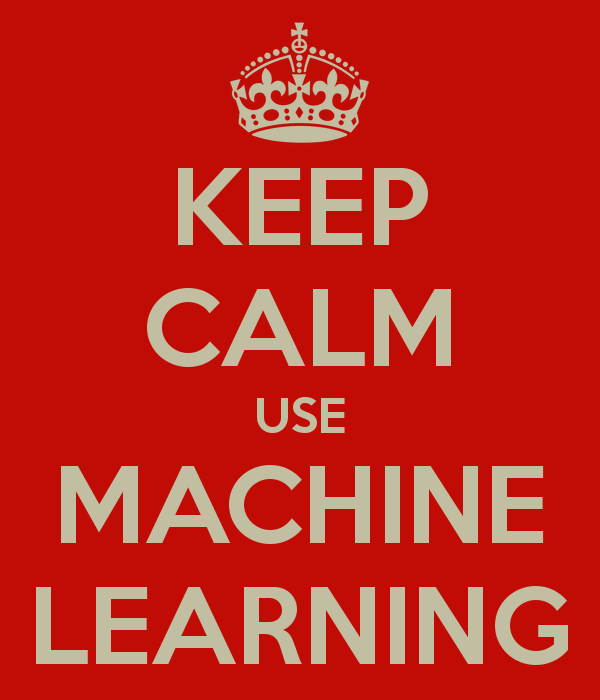
\includegraphics[width=0.5\textwidth]{machine_learning_logo.png}
  \end{figure}
\end{frame}

\begin{frame}[allowframebreaks]
\frametitle{References}
\footnotesize
\bibliographystyle{apacite}
\bibliography{../dlworkshopref}
\end{frame}

\end{document}
%%% Local Variables:
%%% mode: latex
%%% TeX-master: t
%%% End:
